\graphicspath{{./figures}}

\section{PocketQube Unit}
A block diagram of the system components for the PocketQube unit is shown in Figure \ref{fig:pqunit_system}.

\begin{figure}[!htb]
  \centering
  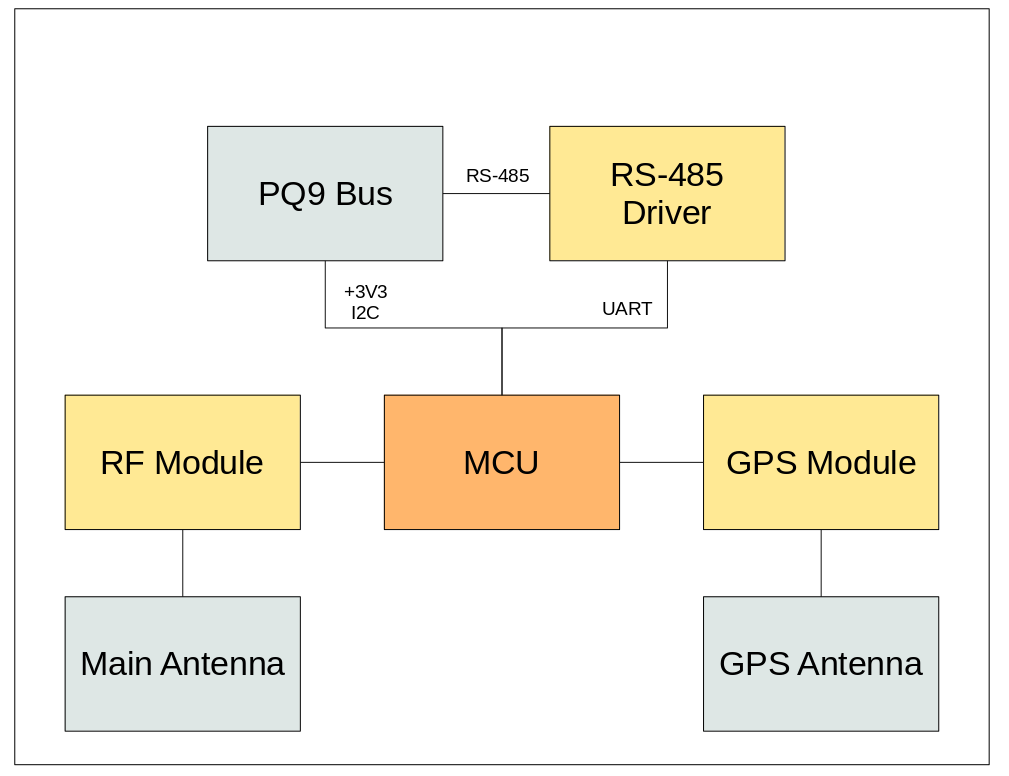
\includegraphics[width=0.6\textwidth]{pqunit_system}
  \caption{PocketQube Unit System Diagram}
  \label{fig:pqunit_system}
\end{figure}

This unit is relatively simple in comparison to the ground station. The unit consists of an RF section, and a GPS section. The system will be powered via the +3V3 on the PocketQube bus. An integrated GPS module, as well as RF module, should be included. Further, an RS-485 line transceiver should be included to cater for the RS-485 protocol, which will likely connect to the MCU via UART.